\section{Formatierte Textinhalte}

Die Aufgaben und Korrektur-Kommentare sollen durch formatierten Text strukturiert dargestellt werden.
Dazu wird die bereits angesprochene \enquote{ActionText} Bibliothek verwendet, die ebenfalls standardmässig mit Ruby on Rails mitgeliefert wird.
Diese enthält neben einigen praktischen Helpern auch den JS Trix-Editor, der alles von der Formatierung über Links, Zitate und Listen bis hin zu eingebetteten Bildern übernimmt. 

Der vom Trix-Editor generierte Rich-Text-Inhalt wird im HTML-Format gespeichert,und eingebettete Bilder (oder andere Anhänge) werden automatisch durch ActiveStorage verwaltet.

Über den generator-command \mintinline{bash}{rails g action_text:install} werden die notwendigen migrationen erstellt und
der Trix-Editor wird über den yarn JS Package-Manager installiert. Dann 

\begin{figure}[H]
\begin{codebox}
\begin{minted}{ruby}
class Task < ApplicationRecord
  belongs_to :assessment, counter_cache: true
  has_many :solutions, dependent: :destroy
  has_rich_text :body
  
  ...
end
\end{minted}
\end{codebox}
\end{figure}

\begin{figure}[H]
\begin{codebox}
\begin{minted}{ruby}
= simple_form_for([@assessment, @task]) do |f|
    = f.input :body, as: :rich_text_area
\end{minted}
\end{codebox}
\end{figure}

\begin{figure}[H]
  \centering
  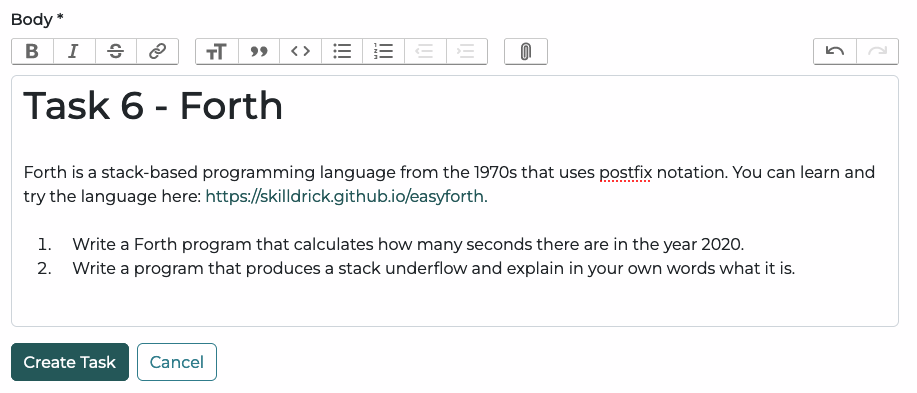
\includegraphics[width=14cm]{images/trix.png}
  \caption{Der ActionText \emph{trix} Rich-Text-Editor}
\end{figure}
